\documentclass{standalone}
\usepackage{amsmath}
\usepackage[dvipsnames]{xcolor}
\usepackage{tikz} 
\usetikzlibrary{arrows, decorations.markings,decorations.pathreplacing,angles,quotes}
\usepackage{microtype}
\usepackage{fourier}

\definecolor{nblue}{RGB}{31, 119, 180}

\begin{document}

\begin{tikzpicture}
   		\node[anchor=south west,inner sep=0] (Bild) at (0,0) {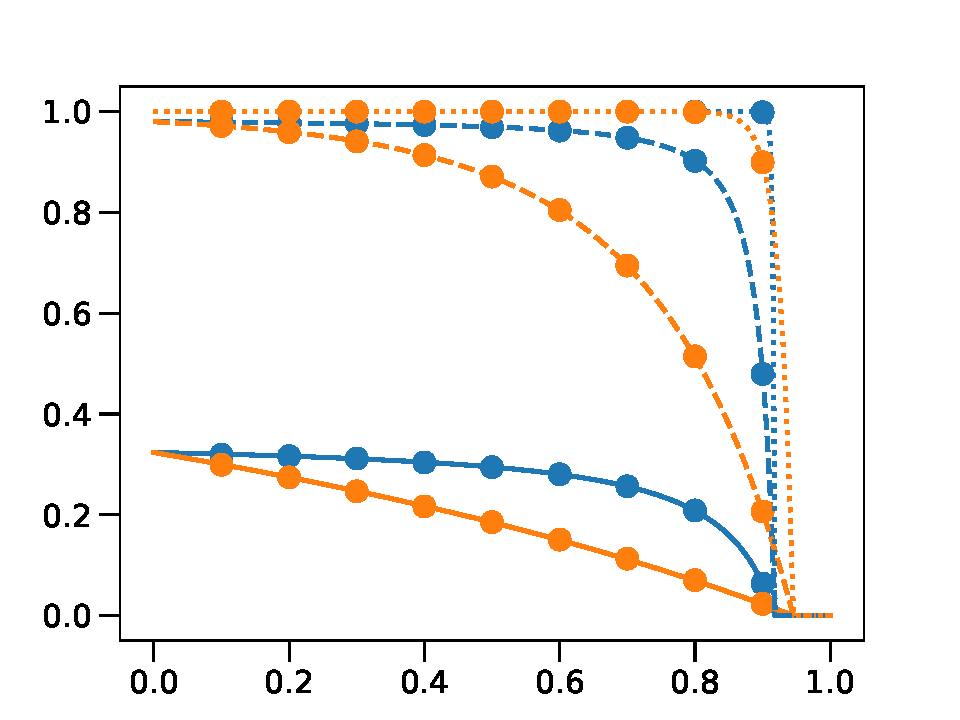
\includegraphics[scale=0.39]{figS6a_blank.pdf}};
   		\begin{scope}[x=(Bild.south east),y=(Bild.north west)]
        	\draw (0.55,-0.035) node {antiviral drug efficacy $\varepsilon_j$};
        	\draw (0.01,0.5) node [rotate=90] {establishment probability $\varphi$};
        	\draw[nblue,thick] (0.175,0.15) -- node[right=6pt] {\scriptsize \color{black} reducing viral production $p$} (0.225,0.15);
        	\draw[orange,thick] (0.175,0.2) -- node[right=6pt] {\scriptsize \color{black} reducing infectivity $\beta$} (0.225,0.2);
        	\draw[black,thick] (0.175,0.7) -- node[right=6pt] {\scriptsize \color{black} $V_0=1$} (0.225,0.7);
        	\draw[black,thick,dashed] (0.175,0.63) -- node[right=6pt] {\scriptsize \color{black} $V_0 = 10$} (0.225,0.63);
        	\draw[black,thick,dotted] (0.175,0.56) -- node[right=6pt] {\scriptsize \color{black} $V_0 = 100$} (0.225,0.56);
    		\end{scope}
\end{tikzpicture}

\end{document}